\section{Charge Carriers and Doping}
We start learning about resistors, capacitors, and inductors from earlier courses such as EECS 16A and 16B. With more components like transistors, diodes, and op-amps (which are all based on semiconductors), we are able to expand upon circuit design. We need to understand semoconductor physics in order to understand how these components operate.
\begin{center}
    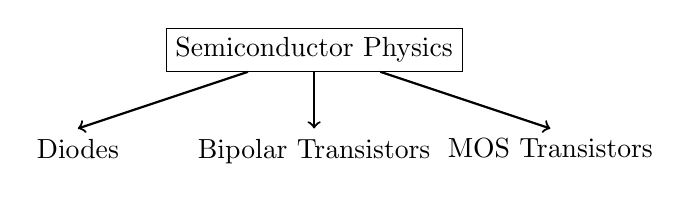
\begin{tikzpicture}
        \node[draw, align=center] (text) {Semiconductor Physics};
        \draw[->, thick] (text) -- ++(0,-1) node[below] {Bipolar Transistors};
        \draw[->, thick] (text) -- ++(-3,-1) node[below] {Diodes};
        \draw[->, thick] (text) -- ++(3,-1) node[below] {MOS Transistors};
    \end{tikzpicture}
\end{center}


Doping is one method that we use in semiconductor devices to introduce more or fewer electrons, which change conductivity. The following materials are commonly used:
\begin{pline}
    \item Group III elements: $\rightarrow$ acceptors
    \item Group IV elements: germanium and silicon
    \item Group V elements: $\rightarrow$ donors
\end{pline}

\subsection{Practice Problems}

\subsection{Sources}
\begin{itemize}
    \item \href{https://www.youtube.com/watch?v=yQDfVJzEymI}{\textcolor{blue}{Razavi Electronics 1, Lec 1, Intro., Charge Carriers, Doping}}
    \item Sedra, Adel S., et al. Microelectronic Circuits. Oxford University Press, 2021
\end{itemize}

